\documentclass[article]{uom-coursework}
% \usepackage[showframe]{geometry}
\usetikzlibrary{automata, positioning, arrows, arrows.meta}

\counterwithout{section}{chapter}

% Biblography
% \addbibresource{dsa.bib}

\title{Compiler Theory and Practice}
\tagline{Coursework}
\author{Juan Scerri}
\authorid{123456A}
\courseworkname{Some Degree}
\doctype{coursework}
\courseworkdate{\monthyeardate\today}
\subjectcode{CPS2000}


\begin{document}

%----------------------------------
%	Front Matter
%----------------------------------

\pagestyle{umpage}

\frontmatter

\maketitle % Print the title page

\tableofcontents % Print the table of contents

\clearpage

\lstlistoflistings

\clearpage

\mainmatter

\chapter*{Report}
\label{chap:report}
\addcontentsline{toc}{chapter}{\nameref{chap:report}}

\section{Lexer}


\tikzset{
node distance=2cm, % specifies the minimum distance between two nodes. Change if necessary.
every state/.style={thick, fill=gray!10}, % sets the properties for each ’state’ node
initial text=$\text{start}$, % sets the text that appears on the start arrow
}

So, we'll be using the following micro-syntax:

So, we'll also be using a set of categories as our
language. Some categories are complete types
in their own right. These types will be the following:

Let $\mathfrak{U}$ be the set of all unicode characters.

\begin{itemize}
    \item $L \coloneq \{
        \texttt{A},\ldots,\texttt{Z},\texttt{a},\ldots,\texttt{z}\}$
    \item $D \coloneq \{\texttt{0},\ldots,\texttt{9}\}$
    \item $H \coloneq \{\texttt{A},\ldots,\texttt{F},\texttt{a},\ldots,\texttt{f}\} \cup D$
    \item $S \coloneq \{\alpha \in \mathfrak{U} \colon \alpha\ \text{is whitespace}\}\setminus\{\texttt{LF}\}$
\end{itemize}

$\Sigma = L \cup D \cup S \cup
\{\texttt{.},\texttt{\#},\texttt{\_},\texttt{(},\texttt{)},\texttt{[},\texttt{]},\texttt{\{},\texttt{\}},\texttt{*},\texttt{/},\texttt{+},\texttt{-},\texttt{<},\texttt{>},\texttt{=},\texttt{!},\texttt{,},\texttt{:},\texttt{;},\texttt{LF}\}$

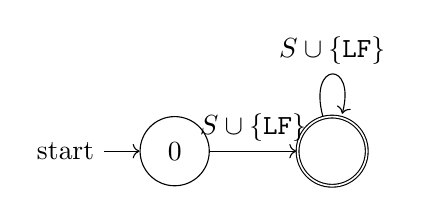
\begin{tikzpicture}
\node[state,initial] (q1) {$0$};
\coordinate[right of=q1] (tq1) {};
\node[state, right of=tq1, accepting] (q2) {};
\draw
    (q1) edge[above, ->] node{$S\cup\{\texttt{LF}\}$} (q2)
    (q2) edge[loop above, ->] node{$S\cup\{\texttt{LF}\}$} (q2);
\end{tikzpicture}

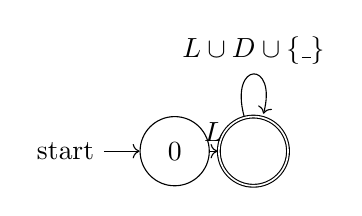
\begin{tikzpicture}
\node[state,initial] (q1) {$0$};
\node[state, right of=q1, accepting] (q2) {};
\draw
    (q1) edge[above, ->] node{$L$} (q2)
    (q2) edge[loop above, ->] node{$L \cup D \cup \{\texttt{\_}\}$} (q2);
\end{tikzpicture}

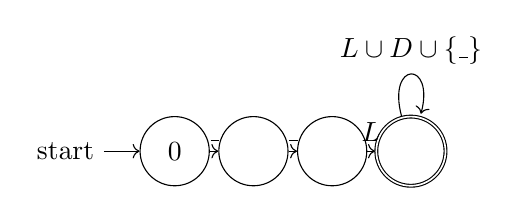
\begin{tikzpicture}
\node[state,initial] (q1) {$0$};
\node[state, right of=q1] (q2) {};
\node[state, right of=q2] (q3) {};
\node[state, right of=q3, accepting] (q4) {};

\draw
    (q1) edge[above, ->] node{\texttt{\_}} (q2)
    (q2) edge[above, ->] node{\texttt{\_}} (q3)
    (q3) edge[above, ->] node{$L$} (q4)
    (q4) edge[loop above, ->] node{$L \cup D \cup \{\texttt{\_}\}$} (q4);
\end{tikzpicture}


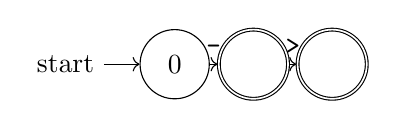
\begin{tikzpicture}
\node[state,initial] (q1) {$0$};
\node[state, right of=q1, accepting] (q2) {};
\node[state, right of=q2, accepting] (q3) {};
\draw
    (q1) edge[above, ->] node{\texttt{-}} (q2)
    (q2) edge[above, ->] node{\texttt{>}} (q3);
\end{tikzpicture}

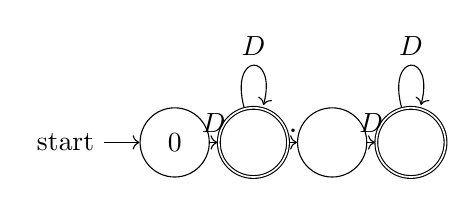
\begin{tikzpicture}
\node[state,initial] (q1) {$0$};
\node[state, right of=q1, accepting] (q2) {};
\node[state, right of=q2] (q3) {};
\node[state, right of=q3, accepting] (q4) {};
\draw
    (q1) edge[above, ->] node{$D$} (q2)
    (q2) edge[loop above, ->] node{$D$} (q2)
    (q2) edge[above, ->] node{\texttt{.}} (q3)
    (q3) edge[above, ->] node{$D$} (q4)
    (q4) edge[loop above, ->] node{$D$} (q4)
    ;
\end{tikzpicture}

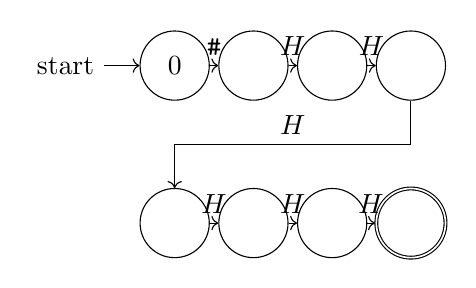
\begin{tikzpicture}
\node[state,initial] (q1) {$0$};
\node[state, right of=q1] (q2) {};
\node[state, right of=q2] (q3) {};
\node[state, right of=q3] (q4) {};

\coordinate[below of=q1] (bq1) {};
\coordinate[below of=q4] (bq4) {};

\node[state, below of=bq1] (q5) {};
\node[state, right of=q5] (q6) {};
\node[state, right of=q6] (q7) {};
\node[state, right of=q7, accepting] (q8) {};
\draw
    (q1) edge[above, ->] node{\texttt{\#}} (q2)
    (q2) edge[above, ->] node{$H$} (q3)
    (q3) edge[above, ->] node{$H$} (q4)
    (q4) -- (bq4)
    (bq4) edge[above] node{$H$} (bq1)
    (bq1) edge[->] (q5)
    (q5) edge[above, ->] node{$H$} (q6)
    (q6) edge[above, ->] node{$H$} (q7)
    (q7) edge[above, ->] node{$H$} (q8)
    ;
\end{tikzpicture}

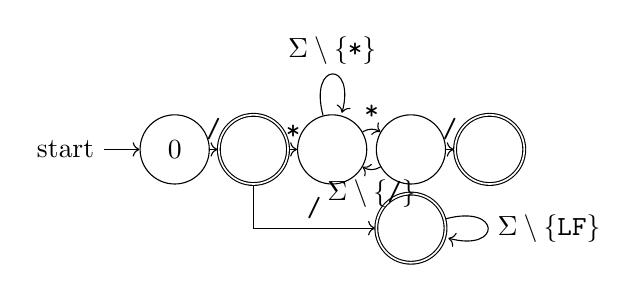
\begin{tikzpicture}
\node[state,initial] (q1) {$0$};
\node[state, right of=q1,accepting] (q2) {};

\coordinate[below of=q2] (bq2) {};

\node[state, right of=q2] (q4) {};
\node[state, right of=q4] (q5) {};
\node[state, right of=q5,accepting] (q6) {};

\node[state, below of=q5, accepting] (q3) {};


\draw
    (q1) edge[above, ->] node{\texttt{/}} (q2)
    (q2) -- (bq2)
    (bq2) edge[above, ->] node{\texttt{/}} (q3)
    (q3) edge[loop right, ->] node{$\Sigma \setminus \{\texttt{LF}\}$} (q3)
    (q2) edge[above, ->] node{\texttt{*}} (q4)
    (q4) edge[loop above, ->] node{$\Sigma \setminus \{\texttt{*}\}$} (q4)
    (q4) edge[above, bend left, ->] node{\texttt{*}} (q5)
    (q5) edge[below, bend left, ->] node{$\Sigma \setminus \{\texttt{/}\}$} (q4)
    (q5) edge[above, ->] node{\texttt{/}} (q6)
    ;
\end{tikzpicture}

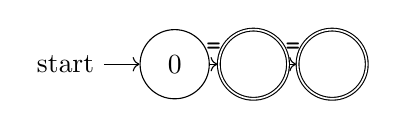
\begin{tikzpicture}
\node[state,initial] (q1) {$0$};
\node[state, right of=q1, accepting] (q2) {};
\node[state, right of=q2, accepting] (q3) {};
\draw
    (q1) edge[above, ->] node{\texttt{=}} (q2)
    (q2) edge[above, ->] node{\texttt{=}} (q3);
\end{tikzpicture}

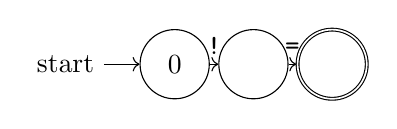
\begin{tikzpicture}
\node[state,initial] (q1) {$0$};
\node[state, right of=q1] (q2) {};
\node[state, right of=q2, accepting] (q3) {};
\draw
    (q1) edge[above, ->] node{\texttt{!}} (q2)
    (q2) edge[above, ->] node{\texttt{=}} (q3);
\end{tikzpicture}

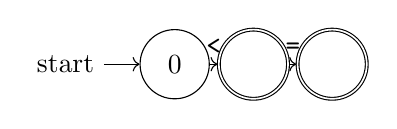
\begin{tikzpicture}
\node[state,initial] (q1) {$0$};
\node[state, right of=q1, accepting] (q2) {};
\node[state, right of=q2, accepting] (q3) {};
\draw
    (q1) edge[above, ->] node{\texttt{<}} (q2)
    (q2) edge[above, ->] node{\texttt{=}} (q3);
\end{tikzpicture}

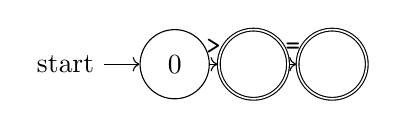
\begin{tikzpicture}
\node[state,initial] (q1) {$0$};
\node[state, right of=q1, accepting] (q2) {};
\node[state, right of=q2, accepting] (q3) {};
\draw
    (q1) edge[above, ->] node{\texttt{>}} (q2)
    (q2) edge[above, ->] node{\texttt{=}} (q3);
\end{tikzpicture}


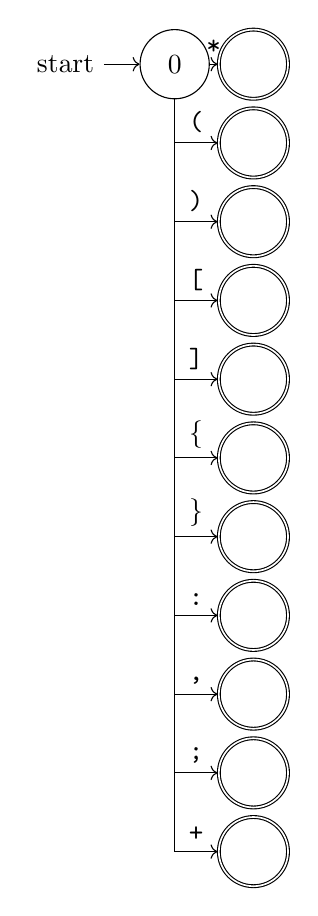
\begin{tikzpicture}
\node[state,initial] (q1) {$0$};

\coordinate[below of=q1] (q3p) {};
\coordinate[below of=q3p] (q4p) {};
\coordinate[below of=q4p] (q5p) {};
\coordinate[below of=q5p] (q6p) {};
\coordinate[below of=q6p] (q7p) {};
\coordinate[below of=q7p] (q8p) {};
\coordinate[below of=q8p] (q9p) {};
\coordinate[below of=q9p] (q10p) {};
\coordinate[below of=q10p] (q11p) {};
\coordinate[below of=q11p] (q12p) {};

\node[state, right of=q1, accepting] (q2) {};
\node[state, below of=q2, accepting] (q3) {};
\node[state, below of=q3, accepting] (q4) {};
\node[state, below of=q4, accepting] (q5) {};
\node[state, below of=q5, accepting] (q6) {};
\node[state, below of=q6, accepting] (q7) {};
\node[state, below of=q7, accepting] (q8) {};
\node[state, below of=q8, accepting] (q9) {};
\node[state, below of=q9, accepting] (q10) {};
\node[state, below of=q10, accepting] (q11) {};
\node[state, below of=q11, accepting] (q12) {};

\draw
    (q1) -- (q3p)
    (q3p) -- (q4p)
    (q4p) -- (q5p)
    (q5p) -- (q6p)
    (q6p) -- (q7p)
    (q7p) -- (q8p)
    (q8p) -- (q9p)
    (q8p) -- (q9p)
    (q8p) -- (q9p)
    (q9p) -- (q10p)
    (q10p) -- (q11p)
    (q11p) -- (q12p)
    ;

\draw
    (q1)  edge[above, ->] node{\texttt{*}} (q2)
    (q3p) edge[above, ->] node{\texttt{(}} (q3)
    (q4p) edge[above, ->] node{\texttt{)}} (q4)
    (q5p) edge[above, ->] node{\texttt{[}} (q5)
    (q6p) edge[above, ->] node{\texttt{]}} (q6)
    (q7p) edge[above, ->] node{\texttt{\{}} (q7)
    (q8p) edge[above, ->] node{\texttt{\}}} (q8)
    (q9p) edge[above, ->] node{\texttt{:}} (q9)
    (q10p) edge[above, ->] node{\texttt{,}} (q10)
    (q11p) edge[above, ->] node{\texttt{;}} (q11)
    (q12p) edge[above, ->] node{\texttt{+}} (q12)
    ;
\end{tikzpicture}


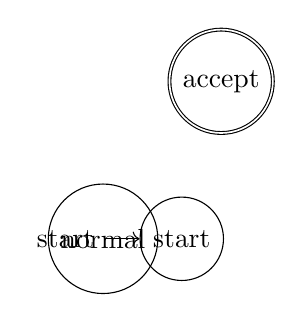
\begin{tikzpicture}
\node[state] (q1) {normal};
\node[state, initial, right of=q1] (q2) {start};
\node[state, accepting] at (1.5, 2) (q3) {accept};
\end{tikzpicture}

\section{Attributions}

\begin{itemize}
    \item Sandro Spina for the brilliant description of table-driven lexers
    \item Robert Nystrom and his great book Crafting Intepreters for a great
        outline for parsing and error recovery/management for languages
        which support exceptions
\end{itemize}


\end{document}
